\documentclass[10pt]{report}
\usepackage[margin=2cm]{geometry}
\usepackage{fontspec}
\usepackage{lmodern}
\usepackage{hyperref}
\usepackage{graphicx}
\usepackage{xcolor}
\usepackage{menukeys}
\usepackage{amsmath}
\hypersetup{
    colorlinks,
    citecolor=red,
    filecolor=black,
    linkcolor=black,
    urlcolor=blue
}
\usepackage{minted}

\graphicspath{{./assets}}
\begin{document}

\begin{titlepage}
\begin{center}
        \pagebreak

        \hspace{0pt}
        \vfill
        {\fontsize{32pt}{10pt}\selectfont Mining Massive Datastructures}\\
        \vspace{2cm}
        {\fontsize{23pt}{2pt}\selectfont \textsc{Assignment : 1}}\\
        
        \vspace{3cm}
        \textsc{\Large Assigned by} \\

        {\large Dr. Subrat K Dash \\
        Associate Professor - Department of CSE \\
        \vspace{0.3cm}
        The LNM Institute of Information Technology, Jaipur} \\
        \vspace{0.7cm}
        \textbf{\today}


        \vspace*{\fill}

        {\fontsize{11pt}{10pt}\selectfont
        \begin{tabular}{rl}
                Shivam Saraswat & 18ucc167 \\
                Manas Singh & 18ucs016 \\
                Gaurav Gupta & 18ucs214
        \end{tabular}}

\end{center}
\end{titlepage}
\pagenumbering{gobble}
\tableofcontents
\clearpage
\pagenumbering{arabic}
\setlength{\parindent}{0pt}
\section{Setup and Installation}
\subsection{Installing Hadoop}
\textbf{Platform:}~{Linux kali 5.10.0-kali3-amd64 \#1 SMP Debian 5.10.13-1kali1 (2021-02-08) x86\_64 GNU/Linux}\\

We set up a \href{https://hadoop.apache.org/docs/stable/hadoop-project-dist/hadoop-common/SingleCluster.html}{single~node~cluster}.\\
Java JDK 15 was a dependency already met by our system.\\
Next, we did not follow the documentation because we intended to use the \href{https://intellij.org}{IntelliJ IDE}. The next section talks about setting up IntelliJ for Hadoop projects.
\
\subsection{IntelliJ \textit{for} Hadoop}
\vspace{0.5cm}
\textbf{Step 1 :} Create a new project and add the following code into a new class \textbf{WordCount.java}.\\

%codeblock
\inputminted[frame=lines]{java}{src/WordCount.java}

\textbf{Step 2 :} Go to \menu{File > Project Structure > Dependencies > +}, and click on \textbf{JARs or Directories} option.
\begin{figure}[h]
        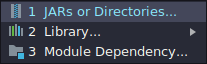
\includegraphics[height=2cm]{JAR.png}
        \centering
        \caption{Select JARs and Directories}
        \centering
\end{figure}
\\

\label{step3}\textbf{Step 3 :} Next Go to \menu{Run > Edit Configurations... > Application > +}, and add arguments in the following format.
\begin{figure}[h]
        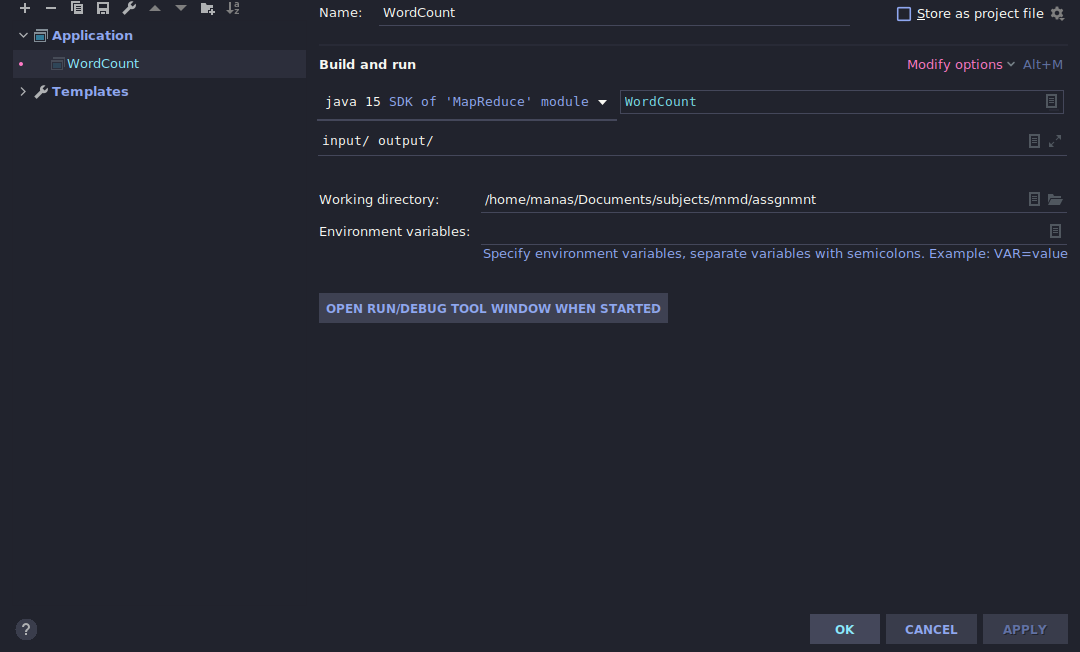
\includegraphics[height=8cm]{arguments.png}
        \centering
        \caption{Program Arguments}
        \centering
\end{figure}
\clearpage

\textbf{Step 4 :} Go to \textit{share/hadoop} and select all the files by holding down \keys{\shift}.
\begin{figure}[h]
        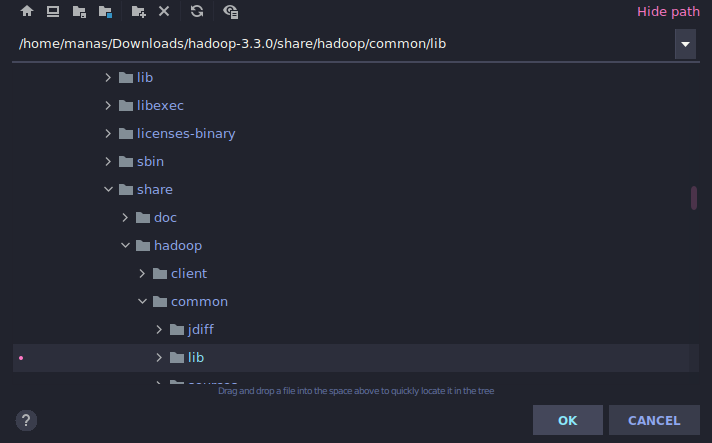
\includegraphics[height=8cm]{dependency1.png}
        \centering
        \caption{share/hadoop}
        \centering
\end{figure}
\\

\textbf{Step 5 :} Go to \textit{share/hadoop/common} and select the \textbf{lib} directory.
\begin{figure}[h]
        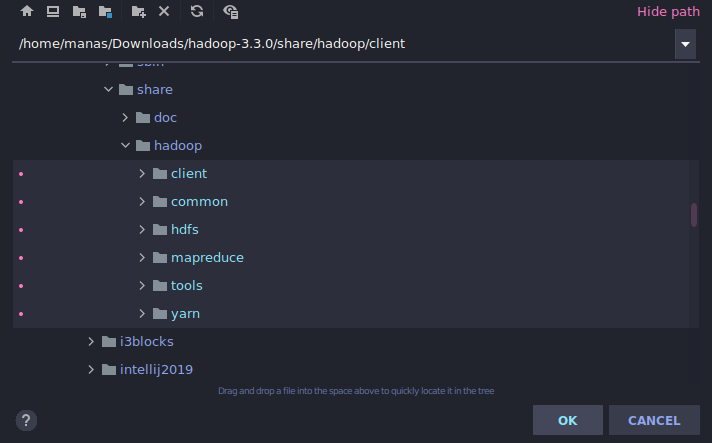
\includegraphics[height=8cm]{dependency2.png}
        \centering
        \caption{share/hadoop/common}
        \centering
\end{figure}
\clearpage

\textbf{Step 6 :} If you did everything right, it will look something like this:
\begin{figure}[h]
        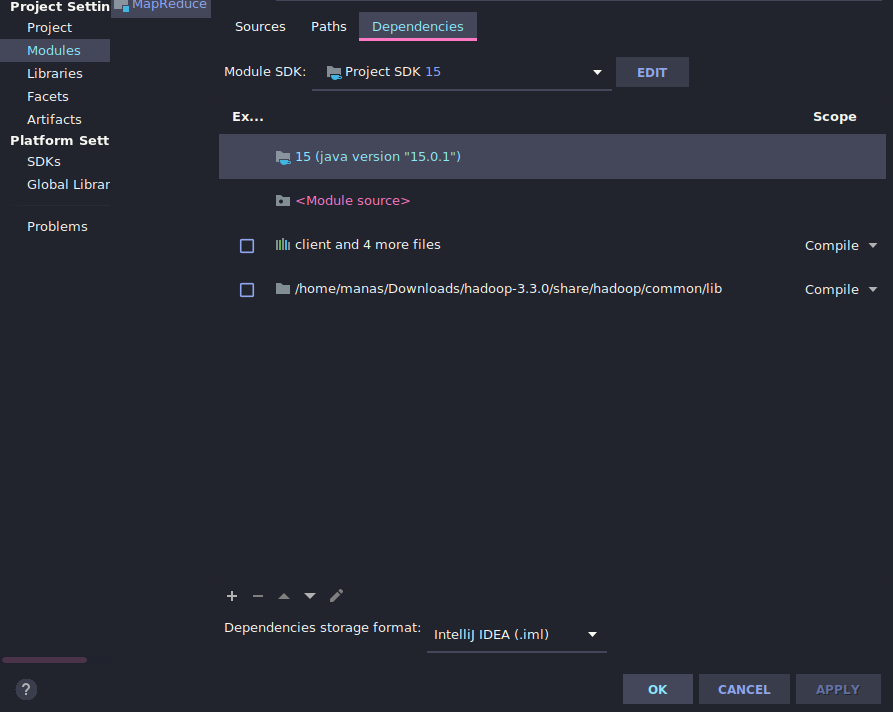
\includegraphics[height=8cm]{dependency.png}
        \centering
        \caption{Added dependencies}
        \centering
\end{figure}
\\

\textbf{Step 7 :} Copy your text file to \textbf{input} directory. In our case \textbf{pride\_and\_prejudice.txt}.
\\

\textbf{Step 8 :} Add the roll numbers of the team members.

\begin{verbatim}
cat >> input/pride_and_prejudice.txt
CSE3152 18ucc167
CSE3152 18ucs016
CSE3152 18ucs214
^C
\end{verbatim}
\clearpage

\section{Building and Running}
\subsection{First Build}

Go ahead and hit \textbf{Build and Run} from the menu bar.

If everything works fine, you will get an output like this:

\begin{figure}[h]
        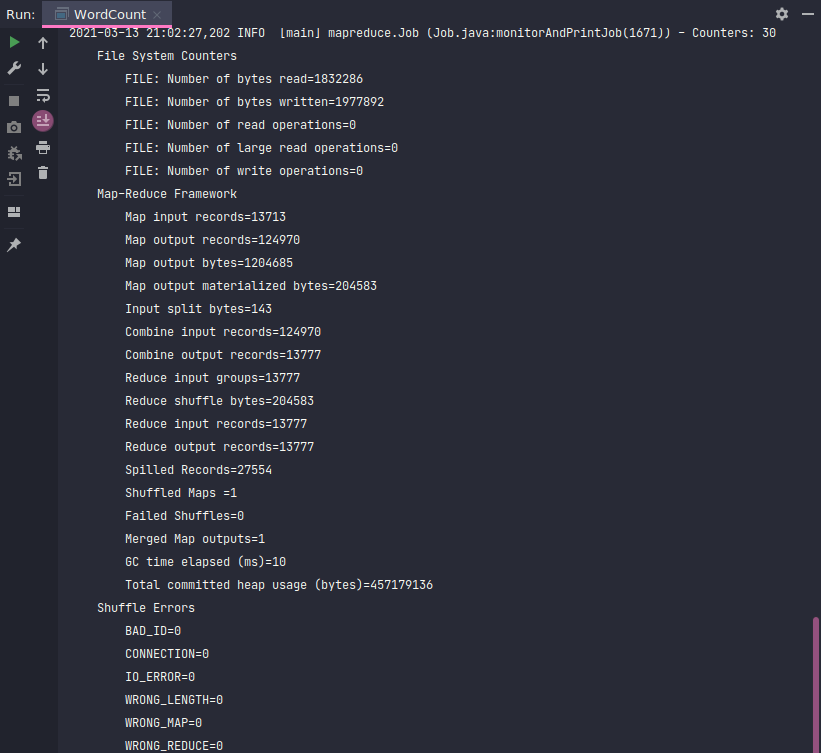
\includegraphics[width=15cm]{MapReduceTask.png}
        \centering
        \caption{MapReduce statistics}
        \centering
\end{figure}
\clearpage

\subsection{Output}
A directory by the name of \textbf{output} would be created automatically, each time you run the program. If you want to re-run it,
you need to delete the directory, or specify another directory in the arguments by following \hyperref[step3]{Step 3}.

The final file structure would look something like this:
\begin{figure}[h]
        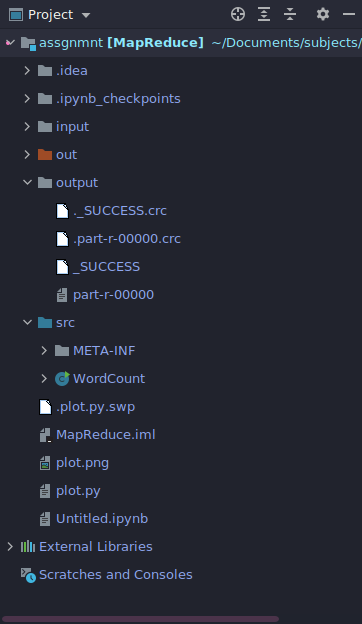
\includegraphics[width=10cm]{FileStructure.png}
        \centering
        \caption{Project File Structure}
        \centering
\end{figure}
\clearpage

\subsection{Artifacts}

Now to make this software portable you might want to create an artifact. For
that go to \menu{File > Project Structure > Artifacts} and add a new artifact
corresponding to \textbf{WordCount.java}. Go to \textbf{Build} and click on
\textbf{Build Artifacts}. From now on you could directly invoke the JAR in the
following manner.

\begin{verbatim}
bin/hadoop jar WordCount.jar input/ output/
\end{verbatim}

\begin{figure}[h]
        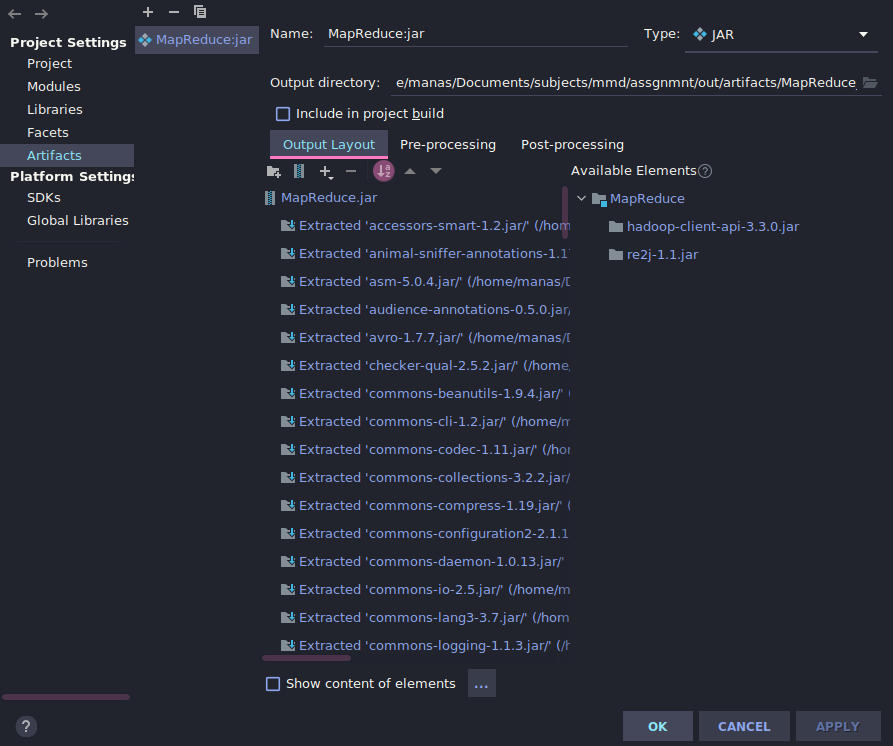
\includegraphics[height=15cm]{artifact.png}
        \centering
        \caption{Artifacts Window}
        \centering
\end{figure}
\clearpage

\section{Analyzing and Plots}
We analyzed the output file \textbf{output/part-r-00000} and made a plot of the
last 50 highest frequency words, and added our own roll numbers for authententicity.

\begin{figure}[h]
        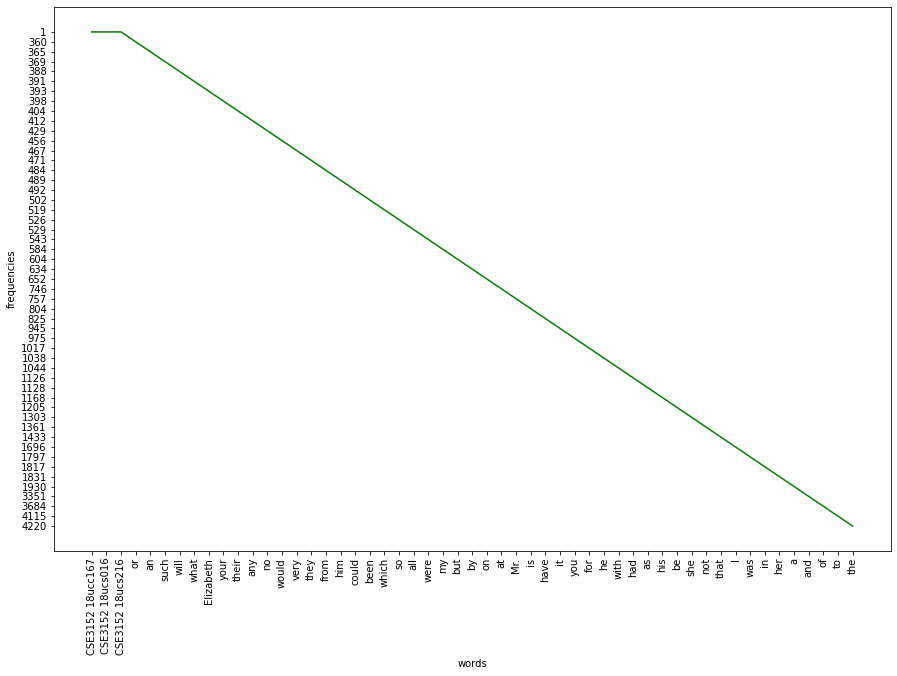
\includegraphics[width=15cm]{plot.png}
        \centering
        \caption{Words vs Frequencies}
        \centering
\end{figure}

%codeblock
\inputminted[frame=lines]{python}{plot.py}

\section{Files and Source}

\url{https://drive.google.com/drive/folders/1bmPB2YIjPwCezrD71AA7GhtOE801Q6Gj?usp=sharing} \\

This report was submitted with all the files itself in ZIP format. \\

The Github repository will go public post the midnight submission deadline at \href{https://github.com/kingmanas/MapReduce}{github.com/kingmanas/MapReduce} \\

Link to pride\_and\_prejudice.txt : \url{http://gutenberg.org/ebooks/42671} \\

\textbf{Apache Tutorials:} \\

Setting up Hadoop : \url{https://hadoop.apache.org/docs/stable/hadoop-project-dist/hadoop-common/SingleCluster.html} \\
Map Reduce in Hadoop : \url{https://hadoop.apache.org/docs/stable/hadoop-mapreduce-client/hadoop-mapreduce-client-core/MapReduceTutorial.html#Example:_WordCount_v1.0]} \\

\end{document}


